\documentclass{article}
\usepackage[utf8]{inputenc}
\usepackage[english,ngerman]{babel}
%% ========================================================================
%%%% MISC usepackages
%% ========================================================================

%% Chemistry
\usepackage{chemfig,chemmacros}
\chemsetup{modules = all}
\chemsetup[redox]{explicit-sign = true}
\chemsetup[phases]{pos=sub}
%\chemsetup[reactions]{before-tag = {R}, tag-open = [, tag-close = ]}
  
%% Maths
\usepackage{amsmath,amssymb,amsthm,textcomp}

%% Physics
\usepackage{siunitx}

%% Graphics
\usepackage{graphicx}
\usepackage{tikz}
\usepackage{rotating}
%\usepackage{subfig}

%% Tables and Lists
\usepackage{enumerate}
\usepackage{multicol}
\usepackage{geometry}
\usepackage{tabu}
\usepackage{listings}
\usepackage{tabularx}

%% Structures and Style
\usepackage{caption}
\usepackage{subcaption}
\usepackage{booktabs}
\usepackage{colortbl}

\usepackage{xcolor}
\usepackage{xfrac}
\usepackage[export]{adjustbox}[2011/08/13]

\usepackage{booktabs}
\usepackage{float}

\usepackage{fancyhdr}

%% Citing and Settings
\usepackage[backend=biber,
style=numeric,
backref=true, 
natbib=true, %% offering natbib-compatible commands
hyperref=true, %% using hyperref-package references
sorting= none,
doi=true,
maxcitenames=10,
maxbibnames=100,
citestyle=numeric
]{biblatex}

\addbibresource{references.bib}

\usepackage[toc,automake]{glossaries}
\include{abbrevations}
\makeglossaries

\usepackage[colorlinks=true,linkcolor=blue]{hyperref}

%% Figure settings
\renewcommand{\figurename}{Abbildung}
\renewcommand{\tablename}{Tabelle}
\renewcommand{\listfigurename}{Abbildungsverzeichnis}
\renewcommand{\listtablename}{Tabellenverzeichnis}

%% ========================================================================
%%%% Document Information
%% ========================================================================

%% Title
\title{Atommassenbestimmung von Magnesium bzw. der Ladung des Magnesiumions \cite{Versuchsvorschrift}} % Title
\author{Autor: Florian \textsc{Kluibenschedl}} % Author name
\date{Bericht verfasst am: \today} % Date for the report

% Page style - headers
\pagestyle{fancy}
\fancyhf{}
\rhead{PR Allgemeine Chemie A - SS2019}
\lhead{Institut für Allgemeine Chemie - Universität Innsbruck}
\rfoot{Experiment 1 - Seite \thepage}

\begin{document}
  \renewtagform{reaction}[Rgl. ]{}{}
  
  \maketitle % Insert the title, author and date
  
  \begin{center}
    \begin{tabular}{r p{4cm}}
      Versuchsdurchführung am: & 07. März 2019\\ % Date the experiment was performed
      Gruppe, Matrikelnummer: & 3, 11805747 \\
      Lehrveranstaltung: & PR Allgemeine Chemie A \\
      Institut: & Allgemeine, Anorganische und Theoretische Chemie \\
      Assistent: & Kriesche Bernhard % Instructor/supervisor
    \end{tabular}
  \end{center}


  \begin{abstract}
    Die Bestimmung von Atommassen hat historische Bedeutung in der Chemie. Durch Messen der entstandenen Menge an \ch{H2\gas} bei der Reaktion von Magnesium mit \SI[mode=text]{4}{M} \ch{HCl} konnte die Atommasse von \ch{Mg} zu \SI[mode=text]{23.6}{\gram\per\mole} bestimmt werden. Bei gleichem Prinzip der Messung konnte bei angenommen bekannter Molmasse die Stöchiometrie der Reaktionsgleichung verifiziert werden.
  \end{abstract}
  
  \pagebreak 
  
  \section{Theoretische Grundlagen}
  
    \subsection{Motivation} \label{sec:Motivation}
  Bei Magnesium handelt es sich um ein unedles Metall ($E^{0} = -2.36 V$ \cite[S. 881]{PhysicalChemistryAtkings}) und damit um ein gutes Reduktionsmittel, das mit Salzsäure unter Wasserstoffentwicklung reagiert.   

  \begin{reaction}
    Mg\sld{} + $\nu$ H\pch\aq -> Mg\pch[$\nu$] \aq{} + $\nu$ * 1/2 H2\gas{} \label{rec:MagnesiumWasserstoffAllgemein}
  \end{reaction}
  
  Angenommen, es sei bekannt, dass Magnesium als zweifach positiv geladenes Ion vorkommt ($\nu = 2$ in \ref{rec:MagnesiumWasserstoffAllgemein}). Damit ist die Stöchiometrie der obigen Gleichung bekannt und man kann durch Messung der entstehenden Menge an Wasserstoff auf die an der Reaktion beteiligte Stoffmenge an Magnesium schließen. Ist zudem die zu Beginn eingesetzte Masse an Magnesium bekannt, errechnet sich daraus direkt die Molmasse. Nimmt man nun umgekehrt die molare Masse des Magnesiums als bekannt an, kann auf die stöchiometrischen Faktoren und damit die Ionenladung geschlossen werden. 
  
  Beide Größen gleichzeitig zu bestimmen ist mit der beschriebenen Methode nicht möglich, wobei durch einen Blick auf das Periodensystem getrost die Annahme getroffen werden kann, dass $\nu = 2$.
  
    \subsection{Ziel des Experiments}
    
    Auf Basis der obigen Überlegungen ist das Ziel, eine möglichst exakte Bestimmung der Molmasse von Magnesium durchzuführen.
    
  \section{Experimenteller Teil}
  
    \subsection{Verwendete Materialien}
              
      \begin{table}[H]
        \centering
        \caption[Materialienliste, Quelle: Autor]{Auflistung der verwendeten Geräte und Chemikalien}
        \label{tab:Materialien}
        
        \begin{tabular}{@{}ll|ll@{}}
          \toprule
            Geräte & Hersteller & Chemikalie & Hersteller \\ \midrule
            \SI[mode=text]{600}{\milli\litre} Becherglas & DURAN & \ch{Mg}-Streifen & Vorrat \\
            \SI[mode=text,separate-uncertainty=true]{25.000(75)}{\milli\litre} Bürette & BRAND & \SI[mode=text]{4}{M} \ch{HCl} & Vorrat \\
            \SI[mode=text,separate-uncertainty]{10.0(1)}{\milli\litre} Messzylinder & BRAND & deionisiertes \ch{H2O} & Labor \\
            Bindfaden &  &  &  \\
            Thermometer & TFA &  &  \\
            Stativ mit Klammern &  &  &  \\
            \SI[mode=text]{14}{\centi\meter} Geodreieck & ARISTO &  &  \\
            Pinzette &  &  &  \\ \bottomrule
        \end{tabular}
      \end{table}
    
    \pagebreak
    
    \subsection{Versuchsdurchführung} \label{sec:Versuch}
    
    \begin{figure}[h]
      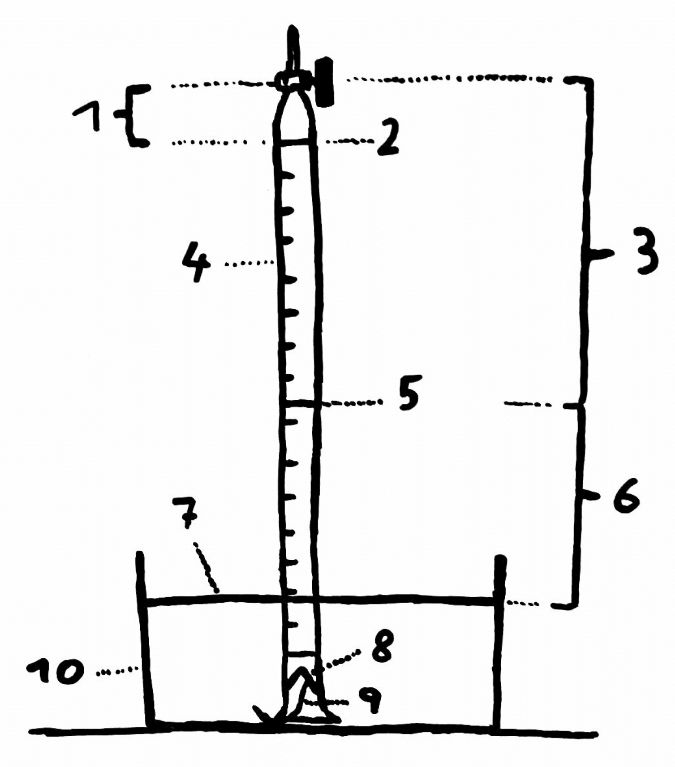
\includegraphics[scale=0.3, center]{Graphiken/Versuchsanordnungen/VersuchsanordnungMagnesium.png} 
      \caption[schematische Versuchsanordnung, Quelle: Autor]{schematische Versuchsanordnung: (1) Totvolumen, (2) \SI[mode=text]{25}{\milli\litre} Marke, (3) Gasraum - gefüllt mit \ch{H2} und \ch{H2O} Dampf, (4) Bürette - mit Klammern an einem Stativ befestigt, (5) Wasserstand in der Bürette, (6) Wassersäule, (7) Flüssigkeitsstand im Becherglas, (8) V-förmig geknichter Magnesiumstreifen, (9) Bindfaden, (10) \SI[mode=text]{600}{\milli\litre} Becherglas}
      \label{fig:Versuchsanordnung}
    \end{figure}
    
    Zu Beginn wurde das Totvolumen der Bürette bestimmt. Dazu wurde diese mit destilliertem Wasser bis zur \SI[mode=text]{25}{\milli\litre} Marke aufgefüllt und anschließend das Wasser in einen \SI[mode=text]{10}{\milli\litre} Messzylinder bis zum Hahn abgelassen und das Volumen notiert. Diese Prozedur wurde 3 mal wiederholt.\\
    
    Der Versuch wurde wie in Abbildung \ref{fig:Versuchsanordnung} dargestellt aufgebaut. Die Bürette wurde mit ca. \SI[mode=text]{25}{\milli\litre} \SI[mode=text]{4}{M} \ch{HCl} gefüllt. Anschließend wurde mit destilliertem Wasser bis zum Bürettenrand aufgefüllt. Beim Auffüllen wurde darauf geachtet, dass es zu einer möglichst geringen Aufwirbelung der Salzsäure kommt, um einem frühzeitigen Reaktionsstart vorzubeugen. Dementsprechend wurde die \ch{HCl} langsam zugegeben. Ein  Magnesiumstreifen bekannter Masse wurde ca. \SI[mode=text]{2}{\centi\meter} in das Wasser eingetaucht. Um ein Absinken zu verhindern, hat man den Streifen V-förmig abgeknickt (um ihn zwischen den Bürettenwänden einzuklemmen) und an einem Bindfaden befestigt. Nach dem Versenken des Magnesiumstreifens mit einer Pinzette wurde die Bürette wieder mit destilliertem Wasser bis zum Rand aufgefüllt. 
    
    Die Reaktion wurde nun gestartet, indem die Bürette mit dem Daumen dicht verschlossen\footnote{dabei wurde darauf geachtet, die Entstehung von Luftblasen zu vermeiden} und verkehrt in das Becherglas getaucht wurde, wie in Abbildung \ref{fig:Versuchsanordnung} gezeigt. Aufgrund der größeren Dichte von Salzsäure (\SI[mode=text]{1.19}{\gram\per\cubic\centi\metre} bei \SI[mode=text]{20}{\degreeCelsius} für eine 37 \%-ige Salzsäure \cite{Salzs}) im Vergleich zu destilliertem Wasser (\SI[mode=text]{0.997}{\gram\per\cubic\centi\metre} bei \SI[mode=text]{20}{\degreeCelsius}) diffundierte diese nach unten und reagierte mit dem Magnesiumstreifen unter Wasserstoffentwicklung. 
    
    Das Ende der Reaktion war erreicht, sobald das gesamte Magnesium reagiert hatte\footnote{anzumerken ist, dass die \ch{HCl} in einem Überschuss zugegeben wurde, um eine möglichst vollständige Reaktion zu ermöglichen}, optisch erkennbar durch ein vollständiges Auflösen. Mithilfe eines Lineals wurde der Abstand zwischen Flüssigkeitsstand in der Bürette und dem Flüssigkeitsstand des Becherglases bestimmt. Durch Ablesen der Markierung in der Bürette konnte unter Berücksichtigung des Totvolumens der Bürette das Volumen an enstandenem Wasserstoff bestimmt werden. Die Temperatur des Wassers wurde mit einem Badthermometer bestimmt.  
     
    \subsection{Auswertung}
    
      Im Folgenden wird eine Beziehung hergeleitet, mit der die gebildete Stoffmenge an Wasserstoff mit den gemessenen Daten berechnet werden kann. 
      
      Das oben skizzierte System erreicht seinen Gleichgewichtszustand, wenn der Innendruck gleich dem Aussendruck ist.
    
      \begin{equation}
        p_{innen} = p_{außen} \label{eq:InnenAussen}
      \end{equation}
    
      Der Innendruck (\ref{eq:Innendruck}) setzt sich zusammen aus dem Dampfdruck des Wassers $p_{\ch{H2O}}$, dem Druck des Wasserstoffs $p_{\ch{H2}}$ und dem hydrostatischen Druck $p_{h}$ (\ref{eq:hydrostatischerDruck}), der vom  verbleibenden Wasser in der Bürette auf das Wasser im Becherglas ausgeübt wird. Der Außendruck entspricht dem Atmosphärendruck $ p_{Atm.}$.
    
      \begin{equation} 
        p_{h} = \rho * g * h \label{eq:hydrostatischerDruck}
      \end{equation} 
    
      \begin{equation}
        p_{innen} = p_{\ch{H2}} + p_{\ch{H2O}} + p_{h} \label{eq:Innendruck}
      \end{equation}
    
      Wasserstoff verhält sich bei den gegebenen Bedingungen wie ein ideales Gas, weswegen die Stoffmenge an Wasserstoff mit der idealen Gasgleichung berechnet werden kann.
    
      \begin{equation}
        n_{\ch{H2}} = \frac{p_{\ch{H2} * V_{Gas}}}{R*T} \label{eq:StoffmengeWasserstoff}
      \end{equation}     
    
      Durch Umformen von \eqref{eq:Innendruck} und einsetzen in \eqref{eq:StoffmengeWasserstoff} erhält man zusammen mit \eqref{eq:hydrostatischerDruck} und \eqref{eq:InnenAussen} einen Ausdruck, mit dem sich die Stoffmenge von Wasserstoff auf Basis der Messdaten berechnen lässt.
    
    
      \begin{equation}
        n_{\ch{H2}} = \frac{V_{Gas}}{R*T} * (p_{Atm.} - \rho * g * h - p_{\ch{H2O}}) \label{eq:Stoffmenge}
      \end{equation}
      
      Die Temperatur von Wasserstoff enstpricht aufgrund seiner hohen Wärmeleitfähigkeit ($\lambda_{\ch{H2}}$ = \SI[mode=text]{0.181}{\watt\per\meter\kelvin} im Vergleich zu $\lambda_{Luft}$ = \SI[mode=text]{0.026}{\watt\per\meter\kelvin} bei \SI[mode=text]{25}{\degreeCelsius} \cite{LambdaHydrogen}) annähernd der gemessenen Wassertemperatur.
    
      \subsubsection{Berechnung der molaren Masse von Magnesium}
    
        Um die molare Masse von Magnesium berechnen zu können, wird die Ladung des Magnesiumions als bekannt vorausgesetzt (wie in \ref{sec:Motivation} bereits erläutert). Es wird angenommen, dass Magnesium als zweifach positives geladenes Ion auftritt ($\nu = 2$). Das Stoffmengenverhältnis von Magnesium und Wasserstoff in Reaktionsgleichung \ref{rec:MagnesiumWasserstoffAllgemein} ist demnach 1:1. Die gesuchte molare Masse lässt sich also wie in \eqref{eq:Molmasse} dargestellt berechnen.
    
        \begin{equation}
          M_{\ch{Mg}} = \frac{m_{\ch{Mg}}}{n_{\ch{H2}}} \label{eq:Molmasse}
        \end{equation}
    
      \subsubsection{Berechnung der Ionenladung von Magnesium}
    
        Es wird vorausgesetzt, dass die molare Masse von Magnesium bekannt ist. Diese wurde der Literatur entnommen. Die Stoffmenge von Magnesium kann also berechnet werden gemäß \eqref{eq:StoffmengeMag}. Da zudem die Stoffmenge von Wasserstoff nach \eqref{eq:Stoffmenge} bekannt ist, lässt sich über das Verhältnis der beiden der gesuchte stöchiometrische Faktor $\nu$ und damit die Ionenladung bestimmen.
    
        \begin{equation}
          n_{\ch{Mg}} = \frac{m_{\ch{Mg}}}{M_{\ch{Mg}}} \label{eq:StoffmengeMag} 
        \end{equation}
    
        \begin{equation}
          \nu = \frac{2*n_{\ch{H2}}}{n_{\ch{Mg}}} = \frac{2*n_{\ch{H2}}*M_{\ch{Mg}}}{m_{\ch{Mg}}} \label{eq:nu}
        \end{equation}
      
    \subsection{Messergebnisse und Literaturwerte}
    
      In Tabelle \ref{tab:Messdaten} sind alle Messwerte angeführt, die im Rahmen der Versuchsdurchführung wie in \ref{sec:Versuch} beschrieben, gemessen wurden. Ebenso sind die verwendeten Literaturwerte derjenigen Messgrößen aufgelistet, die für die Berechnungen notwendig waren.
      
      \begin{table}[H]
        \centering
        \caption[Mess- und Literaturdaten, Quelle: Autor]{Mess- und Literaturdaten}
        \label{tab:Messdaten}
          \begin{tabular}{@{}ll|ll@{}}
            \toprule
             Messgröße & Messwert & Größe bzw. Konstante & Wert \\ \midrule
             $m_{\ch{Mg}}$ & \SI[mode=text]{16.2}{\milli\gram} & R & \SI[mode=text]{8.314}{\joule\per\kelvin\per\mol} \\
             $V_{Gas}$ & \SI[mode=text]{17.0}{\milli\liter} & $M_{\ch{Mg}}$ & \SI[mode=text]{24.31}{\gram\per\mole} \\
             $p_{Atm.}$ & \SI[mode=text]{100570}{\pascal} & g & \SI[mode=text]{9.81}{\meter\per\second\squared} \\
             $T_{Wasser}=T_{\ch{H2}}$ & \SI[mode=text]{19.6}{\degreeCelsius} &  &  \\
             $h$ & \SI[mode=text]{9.3}{\centi\meter} &  &  \\
             $V_{Tot.}$ & \SI[mode=text]{8.4}{\milli\liter} &  &  \\ 
             $p_{\ch{H2O\gas}}$ & \SI[mode=text]{2339.3}{\pascal} &  &  \\ 
             $\rho_{\ch{H2O}}$ & \SI[mode=text]{0.997}{\gram\per\cubic\centi\metre} &  &  \\ \bottomrule
          \end{tabular}
      \end{table}      
      
      Das Totvolumen wurde wie oben beschrieben dreimal bestimmt. Dabei wurde jedesmal ein Wert von \SI[mode=text]{8.4}{\milli\liter} notiert.
      
      Der Wert für den Dampfdruck von Wasser wurde einer Tabelle von internetchemie.info entnommen \cite{Dampfdruck}. 
      
      Der Atomsphärendruck wurde im Internet nachgelesen. Zum Zeitpunkt der Messung zeigte die Messstation der Universität Innsbruck auf der Internetseite zamg.ac.at \cite{zamg} den in Tabelle \ref{tab:Messdaten} angegebenen Druck. Der Wert für die molare Masse von Magnesium wurde \cite{PhysicalChemistryAtkings} entnommen.
      
  \section{Ergebnisse und Diskussion}
  
    Unter der Annahme, dass die Ionenladung von Magnesium bekannt ist ($\nu=2$), errechnet sich durch einsetzen der in Tabelle \ref{tab:Messdaten} angegebenen Werte in \eqref{eq:StoffmengeMag} folgende molare Masse: $M_{\ch{Mg}}=\SI[mode=text]{23.6}{\gram\per\mole}$.
    
    Wird angenommen die molare Masse von Magnesium ist bekannt errechnet sich durch einsetzen in \eqref{eq:nu} folgender Wert für die Ionenladung: $\nu=2.1$. \\
    
    Ein Vergleich mit den Literaturwerten zeigt, dass die Messergebnisse diesen recht nahe kommen. Die entsprechenden Abweichungen: 
    
    \begin{equation}
      \frac{M_{\ch{Mg},exp.}}{M_{\ch{Mg},Lit.}}=0.97
    \end{equation}
      
    \begin{equation}
      \frac{\nu_{exp.}}{\nu_{Lit.}}=1.05
    \end{equation}
    
    Die Abweichungen betragen gerade \SI[mode=text]{5}{\percent}. Ein Grund für den zu niedrigen Wert der Molmasse könnten Luftblasen sein, die sich in der Bürette angesammelt haben. Auch ein Ablesefehler beim Bestimmen des Totvolumens ist denkbar. Eine weitere Möglichkeit ist, dass der Atmosphärendruck im Labor etwas niedriger war wie der Wert der Messstation. Die Annahme, dass die Temperatur von Wasserstoff gleich der Temperatur von Wasser ist, ist vielleicht doch eine zu grobe Abschätzung. Ein frühzeitiger Reaktionsstart, hervorgerufen durch ungewollte Diffusion der \ch{HCl}\footnote{das bestimmte Volumen und die errechnete Stoffmenge wären demnach kleiner und die Molmasse entsprechend größer} kann eher ausgeschlossen werden, da die Molmasse in diesem Falle größer, nicht kleiner werden müsste. \\
    
    Um die Messergebnisse weiter zu verbessern, wird folgendes vorgeschlagen:
    
    \begin{itemize}
      \item den Atmosphärendruck im Labor mithilfe eines Barometers direkt zu bestimmen
      \item eine andere Bürette verwenden, mit der die Bestimmung des Totvolumens leichter möglich ist
      \item eine direkte Messung der Temperatur von Wasserstoff ermöglichen
    \end{itemize}
    
     Zusammenfassend wird das Experiment als recht genau und damit als gelungen betrachtet.
     
  \pagebreak
  
  \listofreactions
  \printbibliography[title=Literaturverzeichnis]
  \listoffigures
  \listoftables
  
\end{document}
